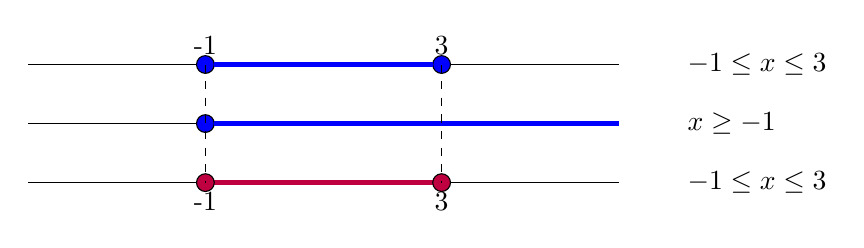
\begin{tikzpicture}[scale=0.75]
    %\draw (-11,0)-- (3,0); %AXIS
    %\foreach \x in {-1} {
    %    \draw (\x,0.5) -- (\x,-0.5) node[below] {$\x$};
    %}
    \draw (-4,1) -- (6,1);
    \draw[fill=blue] (-1,1) circle (0.15) node[above]{-1};
    \draw[fill=blue] (3,1) circle (0.15) node[above]{3};
    \node[anchor=west, right] at (7,1) {$-1 \leq x \leq 3$};
    \draw (-4,0) -- (6,0);
    \draw[fill=blue] (-1,0) circle (0.15);
    \node[anchor=west, right] at (7,0) {$x \geq -1$};
    \draw (-4,-1) -- (6,-1);
    \node[anchor=west, right] at (7,-1) {$-1 \leq x \leq 3$};
    \draw[ultra thick, blue] (-0.85,1) -- (2.85,1);
    \draw[ultra thick, blue] (-0.85,0) -- (6,0);
    \draw[ultra thick, purple] (-1,-1) -- (3,-1);
    \draw[fill=purple] (-1,-1) circle (0.15) node[below]{-1};
    \draw[fill=purple] (3,-1) circle (0.15) node[below]{3};
    \draw[dashed] (-1,1) -- (-1,-1);
    \draw[dashed] (3,1) -- (3,-1);
\end{tikzpicture}